\documentclass{standalone}

\usepackage[dvipsnames]{xcolor}	% This package gives you a set of named colours
\usepackage{tikz}				% This is the TikZ package
							% Note: LaTeX is finicky; you need to put "xcolor" before "tikz"

\begin{document}

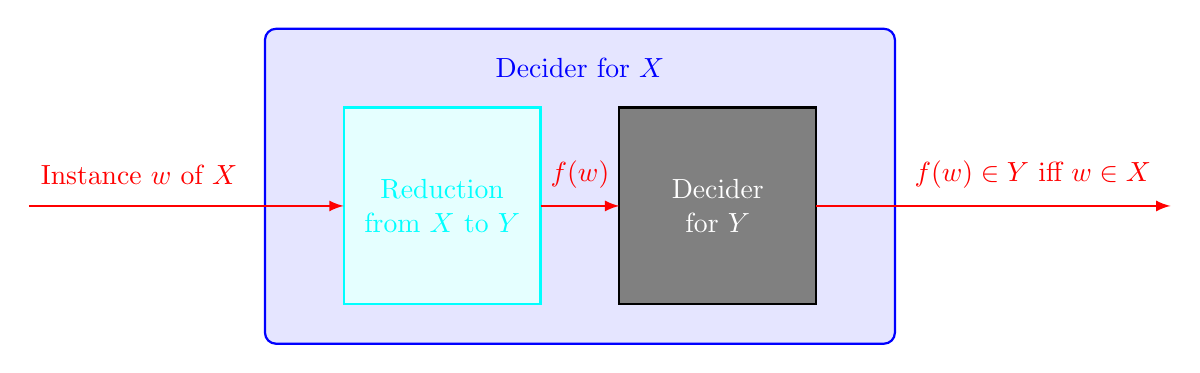
\begin{tikzpicture}
% Drawing a shape
% "draw" = outer (line) colour
% "fill" = inner colour; "blue!10!white" is a way of mixing blue with white with a ratio of 10%
% "thick" = makes the outer line thicker than usual
% "(a,b) rectangle (c,d)" draws a rectangle with bottom-left coordinate (a,b) and top-right coordinate (c,d)
\draw[draw=blue, thick, fill=blue!10!white, rounded corners] (0,0) rectangle (8,4);
\draw[draw=Cyan, thick, fill=Cyan!10!white] (1,0.5) rectangle (3.5,3);
\draw[draw=black, thick, fill=black!50!white] (4.5,0.5) rectangle (7,3);

% Adding a node (for, e.g., text labels)
% "draw=none" = no line will be drawn around the node
% "at (a,b)" positions the node centered on the coordinate (a,b)
% The node's text goes in the {braces}
\node[draw=none, color=blue] at (4,3.5) {Decider for $X$};
\node[draw=none, color=Cyan, text width=2cm, align=center] at (2.25,1.75) {Reduction from $X$ to $Y$};
\node[draw=none, color=white, text width=2cm, align=center] at (5.75,1.75) {Decider for $Y$};

% Defining coordinates and drawing lines
% A coordinate is just a named point in the drawing (e.g., coordinate (1,1.75) is named "A" here)
% "(B) -- (A)" draws a straight line from coordinate B to coordinate A
% Special attributes/properties of the line can be given, like "color=red"
% "-latex" is an arrow type with a triangular head
% You can draw other types of arrows by including, e.g., "->" in the [brackets] instead
\coordinate (A) at (1,1.75);
\coordinate (B) at (-3,1.75);
\draw[-latex, color=red, thick] (B) -- (A);
\node[draw=none, color=red] at (-1.6,2.15) {Instance $w$ of $X$};

\coordinate (C) at (4.5,1.75);
\coordinate (D) at (3.5,1.75);
\draw[-latex, color=red, thick] (D) -- (C);
\node[draw=none, color=red] at (4,2.15) {$f(w)$};

\coordinate (E) at (11.5,1.75);
\coordinate (F) at (7,1.75);
\draw[-latex, color=red, thick] (F) -- (E);
\node[draw=none, color=red] at (9.75,2.15) {$f(w) \in Y$ iff $w \in X$};
\end{tikzpicture}

\end{document}